% Esta configuración tiene desabilitadas las adecuaciones para verso

%---------------------------------------------------------------------------
%    Configuración y Paquetes
%---------------------------------------------------------------------------
\usepackage[utf8]{inputenc} % Escribir caracteres latinos
\usepackage[spanish,mexico,es-nodecimaldot]{babel} % Idioma español mexicano

%------------------------------------------------
%   Márgenes

\usepackage[letterpaper]{geometry}	% Dimensiones del documento
\geometry{
	left = 25mm,
	right = 25mm,
	top = 25mm,
	bottom = 25mm,
}

%------------------------------------------------
%   Tipografía

\usepackage[T1]{fontenc}	% Usar fuentes bonitas
\usepackage{notomath}	% Fuente para Serif
\usepackage{courierten}	% Fuente para Mono
\usepackage{atkinson}	% Fuente Sans Serif (anti dislexia)
\renewcommand*\familydefault{\sfdefault} % Activar Sans Serif

\usepackage{sectsty}			% Paquete para usar el comando allsectionsfont
\allsectionsfont{\rmfamily} 	% Establecer los titulares con la fuente Serif

%------------------------------------------------
%   Párrafos

\renewcommand{\baselinestretch}{1.15} 	% Interlineado
\setlength{\parskip}{8pt} 		% Espacio entre párrafos
\setlength{\parindent}{0pt} 	% Sangria de primer párrafo

\usepackage[defaultlines=3,all]{nowidow} % Evita las líneas huérfanas

\usepackage{setspace} % Definir separaciones
% En este caso, se utilizó para modificar el interlineado en una parte específica.


% Varias columnas

%\usepackage{multicol} % Usar varias columnas
%\setlength{\columnsep}{0.6cm} % Separación entre las columnas

%------------------------------------------------
%   Titulos

\setcounter{secnumdepth}{0} % Hacer que las secciones no se numeren

\usepackage{titlesec} % Para hacer modificaciones en los titulos
% El ajuste se realiza en {izquierda} {anterior} {posterior}
\titlespacing{\section}{0cm}{8pt}{-4pt} % Espaciado de la sección
\titlespacing{\subsection}{0cm}{6pt}{-6pt} % Espaciado de la subsección

%------------------------------------------------
%   Tabla de contenidos

\addto\captionsspanish{ % Modificar subtítulos cambiados por Babel
	\renewcommand{\contentsname}{\begin{center}\rmfamily Cuadros\end{center}}
}

\usepackage{tocloft} % Para personalizar la tabla de contenidos

\renewcommand\cftsecfont{\rmfamily \bfseries \small} % Tamaño de las secciones
\renewcommand\cftsecpagefont{\rmfamily \small} % Tamaño del número de las secciones
\renewcommand\cftsecafterpnum{\vspace{-0.5ex}} % Separación de las secciones

\renewcommand{\cftsecleader}{\cftdotfill{\cftdotsep}} % Añadir puntos

%------------------------------------------------
%   Resaltado y color

\usepackage{xcolor} % Uso de color
\usepackage{soul}	% Hacer resaltados con color

% Comando para resaltar en cualquier color (incluidas combinaciones)
\DeclareRobustCommand{\hlc}[2][yellow]{{%
		\colorlet{foo}{#1}%
		\sethlcolor{foo}\hl{#2}}%
}
% IMPORTANTE, los signos de porcentaje (%) son para evitar espacios indeseados al momento de ejecutar el comando. Por favor, no retirarlos de la definición.

%------------------------------------------------
%   Más utilidades

\usepackage[hidelinks]{hyperref} % Para hacer hipervínculos
\usepackage{ifthen}	% Poder evaluar condicionales

\usepackage{graphicx} 	% Incluir gráficos en el documento
\usepackage{tikz}		% Comandos de dibujo y posicionamiento
\usetikzlibrary{babel,calc} % Librerias para TikZ



%---------------------------------------------------------------------------
%    Macros y definiciones
%---------------------------------------------------------------------------

%   Evitar saltos de página | NO SE USÓ. REMPLAZADO POR MINIPAGE

% \newenvironment{absolutelynopagebreak}
% {\par\nobreak\vfil\penalty0\vfilneg\vtop\bgroup}
% {\par\xdef\tpd{\the\prevdepth}\egroup\prevdepth=\tpd}

%------------------------------------------------
%	Indicaciones ténicas

\newenvironment{tecnico}{
	\vspace{1ex}
	\hspace{\fill}
	\begin{minipage}{6.5cm}
		\setstretch{1.0}
		\setlength{\parskip}{6pt} % Espacio entre párrafos
		
		\begin{flushleft}
			\ttfamily
			\small
}{
		\end{flushleft}
	\end{minipage}
	\hspace{2cm}
	\vspace{1ex}
}	

%------------------------------------------------
%   Acotaciones
\newenvironment{acotado}{
	\begin{rmfamily}\begin{itshape}
}{
	\end{itshape}\end{rmfamily}
}

\newcommand{\acotar}[1]{
	\hspace{7mm} \parbox[t]{25em}{(#1)}
}

%------------------------------------------------
%	Parlamentos
\newenvironment{parla}[2][]{
	\vspace{6pt}
	\begin{minipage}{1\linewidth}
		\setlength{\parskip}{8pt} % Espacio entre párrafos
		
		\hspace{25mm} \textrm{\textbf{#2}} \par \vspace{-11pt}
		\begin{habla}
			\ifthenelse{\not\equal{#1}{}}
			{
				\acotar{#1} \par \vspace{-8pt}
			}{}
		}{
		\end{habla}
	\end{minipage}
	\vspace{-4pt}
}

\newenvironment{habla}{
	\leftskip=10mm 
	\rightskip=10mm
}{\par}

%------------------------------------------------
% Versos y canciones

%\newenvironment{versomio}{
%	\begin{flushleft}
%			\small
%			\setstretch{1.0}
%}{
%	\end{flushleft}
%}
%
%\newenvironment{versomiodo}{
%	\begin{flushleft}
%		\begin{multicols}{2}
%			\small
%			\setstretch{1.0}
%}{
%		\end{multicols}
%	\end{flushleft}
%}

%------------------------------------------------

% Continuación
\newcommand{\cont}{\textbf{\hspace{0.5ex} (cont.)}}

% Resaltar personajes
\newcommand{\personaje}[1]{\emph{\textsf{#1}}}

% Final de un texto
\newcommand{\fintexto}{
	\begin{center}
		\vspace{4em}
		{\large \fontfamily{lmss}\selectfont \bfseries FIN}
	\end{center}
}

% Linea de puntos
\newcommand{\Dotfill}{
	\vspace{-8pt}
	\dotfill
}



%---------------------------------------------------------------------------
%    Portada en tiks
%---------------------------------------------------------------------------

\newcommand{\portada}{
	
	\begin{tikzpicture}[remember picture,overlay]
		\coordinate (title) at ($(current page.north)+(0,-25mm)+(0,10mm)$);
		\coordinate (tituba) at ($(current page.south)+(0,25mm)$);
		
		\node[inner sep=0pt,anchor=north] at (title) {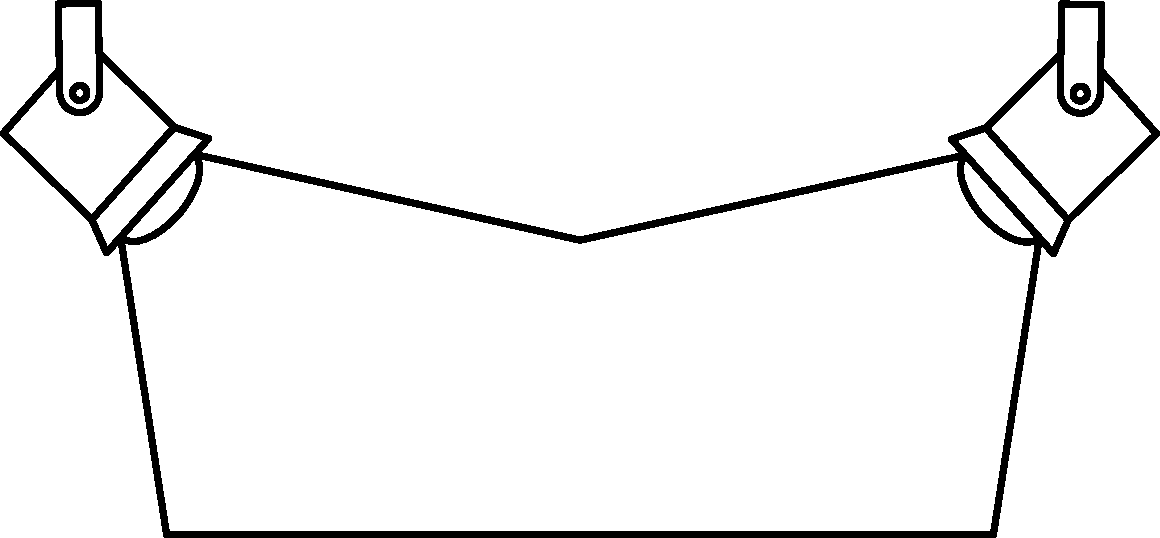
\includegraphics{anexos/vector-portada_Marco_luces.pdf}};
		
		\node[inner sep=0pt,anchor=north] at ([shift={(0,-40mm)}]title) {
			\begin{minipage}[m][50mm]{140mm}
				\setlength{\parskip}{6pt}
				\centering
				
				{\fontsize{35}{42}\selectfont \rmfamily \bfseries\itshape \encabezado}
				
				{\large \rmfamily \scshape \subencabezado}
				
				\vspace{8pt}
				
				{\large \emph{De:} \dramaturgo}
			\end{minipage}
		};
		
		\node[inner sep=0pt,anchor=north] at ([shift={(0,-105mm)}]title) {
			\begin{minipage}{140mm}
				\setlength{\parskip}{10pt}
				\centering
				\large
				
				Dirección: \director
				
				Rev. \fecha
				
			\end{minipage}
		};
		
		\node[inner sep=0pt,anchor=south] at (tituba) {
\includegraphics[height=20mm]{anexos/vector-TITUBA_Expand_1inkB.pdf}};
	\end{tikzpicture}
	
}